% Single-file version for Overleaf: paste into main.tex and compile (pdfLaTeX).
\begin{filecontents*}[overwrite]{refs.bib}
@article{knuth1975alphabeta,
  author  = {Knuth, Donald E. and Moore, Ronald W.},
  title   = {An analysis of alpha-beta pruning},
  journal = {Artificial Intelligence},
  volume  = {6},
  number  = {4},
  pages   = {293--326},
  year    = {1975},
  doi     = {10.1016/0004-3702(75)90019-3}
}

@article{sutton1988td,
  author  = {Sutton, Richard S.},
  title   = {Learning to predict by the methods of temporal differences},
  journal = {Machine Learning},
  volume  = {3},
  number  = {1},
  pages   = {9--44},
  year    = {1988},
  doi     = {10.1007/BF00115009}
}

@article{baxter2000tdleaf,
  author  = {Baxter, Jonathan and Tridgell, Andrew and Weaver, Lex},
  title   = {Learning to play chess using temporal differences},
  journal = {Machine Learning},
  volume  = {40},
  number  = {3},
  pages   = {243--263},
  year    = {2000},
  doi     = {10.1023/A:1007634325138}
}

@article{schaeffer1989history,
  author  = {Schaeffer, Jonathan},
  title   = {The history heuristic and alpha-beta search enhancements in practice},
  journal = {IEEE Transactions on Pattern Analysis and Machine Intelligence},
  volume  = {11},
  number  = {11},
  pages   = {1203--1212},
  year    = {1989},
  doi     = {10.1109/34.42858}
}

@inproceedings{akl1977killer,
  author    = {Akl, Selim G. and Newborn, Monroe M.},
  title     = {The principal continuation and the killer heuristic},
  booktitle = {Proceedings of the 1977 Annual ACM Conference},
  pages     = {466--473},
  year      = {1977}
}

@article{marsland1982pvs,
  author  = {Marsland, T. Anthony and Campbell, Murray},
  title   = {Parallel search of strongly ordered game trees},
  journal = {ACM Computing Surveys},
  volume  = {14},
  number  = {4},
  pages   = {533--551},
  year    = {1982},
  doi     = {10.1145/356893.356895}
}

@article{beyer2002es,
  author  = {Beyer, Hans-Georg and Schwefel, Hans-Paul},
  title   = {Evolution strategies -- A comprehensive introduction},
  journal = {Natural Computing},
  volume  = {1},
  number  = {1},
  pages   = {3--52},
  year    = {2002},
  doi     = {10.1023/A:1015059928466}
}

@misc{stockfish,
  author       = {{The Stockfish developers}},
  title        = {Stockfish: a free and strong {UCI} chess engine},
  howpublished = {\url{https://github.com/official-stockfish/Stockfish}},
  note         = {Accessed November 2026}
}

@misc{gorisanson,
  author       = {gorisanson},
  title        = {quoridor-ai: {Quoridor} {AI} based on {Monte Carlo} tree search},
  howpublished = {\url{https://github.com/gorisanson/quoridor-ai}},
  note         = {MIT licence. Accessed November 2026}
}
\end{filecontents*}
% Wrongway Arena agent report (single-column A4)
\documentclass[11pt,a4paper]{article}

% ---------- encoding & fonts
\usepackage[T1]{fontenc}
\usepackage[utf8]{inputenc}
\usepackage{lmodern}
\usepackage{microtype}

% ---------- layout
\usepackage[a4paper,margin=2.4cm]{geometry}
\usepackage{setspace}\setstretch{1.08}
\usepackage[font=small,labelfont=bf]{caption}
\usepackage{titlesec}
\titlespacing*{\section}{0pt}{1.2ex plus .3ex}{0.6ex}
\titlespacing*{\subsection}{0pt}{1ex plus .2ex}{0.4ex}

% ---------- math, units, tables, figures
\usepackage{amsmath,amssymb}
\usepackage{siunitx}
\sisetup{detect-all, per-mode=symbol}
\usepackage{booktabs,tabularx,multirow}
\usepackage{graphicx}
\usepackage{xcolor}
\usepackage{enumitem}\setlist{noitemsep,topsep=2pt}
\usepackage{tikz}
\usetikzlibrary{arrows.meta,positioning,shapes.geometric}
\usepackage{algorithm}
\usepackage{algpseudocode}

% ---------- references
\usepackage[round,authoryear]{natbib}
\usepackage[hidelinks]{hyperref}
\usepackage{xurl}
\usepackage[capitalise,nameinlink]{cleveref}  % load last

\newcommand{\code}[1]{\texttt{#1}}

\title{\textbf{A Bitboard Alpha-Beta Agent with a Self-Play-Learned Evaluation for Wrongway}\\[2pt]
       \large AI Arena project report}
\author{Team leader: \textless Full name\textgreater{} (\textless Student ID\textgreater)\\
        Members: \textless Full name\textgreater{} (\textless Student ID\textgreater),
        \textless Full name\textgreater{} (\textless Student ID\textgreater)\\[2pt]
        \small Faculty of Information Technology, VNU-HCM University of Science --- November 2026}
\date{}

\begin{document}
\maketitle

% ===== sections/00-abstract.tex =====
\begin{abstract}
\noindent
Wrongway is a two-player race on a $9\times9$ board in which each player may spend up to ten
walls to lengthen the opponent's path. The arena allows one second per move on a Colab CPU, and
the agent must be a single pure-Python file. We built a negamax alpha-beta agent with iterative
deepening. Its evaluation function is a sum of lookup-table entries learned by TD-leaf($\lambda$)
self-play.
Our main finding, which guided most design decisions, is that search depth matters more than
evaluation detail. In a diagnostic run, a fixed depth of 8 plies won 81\% of standard-start games
against the strongest external program we could test, versus 59\% at depth 6. We therefore made
the engine faster: 81-bit bitboards for every breadth-first search, incremental distance updates
after a wall, and Stockfish-style move ordering. Together these give about a 7$\times$ speed-up at
equal depth.
We also removed an odd/even-depth bias of about 9.5 points in the evaluation. The bias had made
the agent change its style depending on the depth it reached.
Self-play learning left one blind spot: walls held in reserve were undervalued against
opponents that keep their walls. Scaling that part of the table by 1.2 raised our standard-start
score against such bots from 0.23 to 0.50 at no measurable cost elsewhere.
The process is logged as 45 numbered experiments covering about 100 hand-designed variants,
about 500 evolutionary weight mutants and six learning runs. Each candidate was judged with
paired, side-swapped games at simulated Colab speed.
In the final evaluation the submitted version scores 0.87 over 160 standard-start games and
0.88 over 640 random-opening games against 16 opponents. The opponents are the course sample
bots, nine team and classmate bots, a bot from another team, an exploit bot and our own earlier
versions.
At simulated grading speed it scores 0.775 from the standard start against the ``Hard'' AI of
wrongway.app, versus 0.17--0.23 for our first trained version.
\end{abstract}

% ===== sections/01-introduction.tex =====
\section{Introduction}
\label{sec:intro}

\paragraph{The game.}
Wrongway is played on a $9\times9$ grid. Player~0 starts at $(8,4)$ and must reach row~0;
player~1 starts at $(0,4)$ and must reach row~8. Player~0 moves first.
On each turn a player does one of three things:
\begin{itemize}
  \item moves one square orthogonally. A player may jump over an adjacent opponent, or step
        diagonally around them when the square behind is blocked;
  \item places one of their ten two-cell walls. Walls may not overlap or cross, and after the
        wall both players must still have a path to their goal;
  \item passes.
\end{itemize}
The first player to reach the goal row wins. A game is drawn after 500 single turns.
A season is a round robin of two games per pair, one on each side, always from the standard
starting position, with 3/1/0 points for a win, draw or loss.
The rules are those of Quoridor plus the \code{pass} action.

\paragraph{Constraints.}
The submission is one Python~3.9+ file using only the standard library. Its function
\code{choose\_action(observation)} returns a move, a wall or a pass. Each call has \SI{1}{\second}
including communication, measured on a Colab CPU. A timeout, an exception or an illegal action
costs the turn. Memory is limited to \SI{128}{\mega\byte}, and the agent cannot rely on global
state because the arena may restart it.

\paragraph{Research question.}
\emph{Under a one-second, pure-Python budget, which combination of search and evaluation gives
the strongest Wrongway agent, and how can candidate versions be compared reliably enough to
choose among them?}

\paragraph{Contributions.}
All code in the submitted file was written by our team, with the help of an AI coding assistant
(\cref{sec:pipeline}).
\begin{itemize}
  \item A negamax alpha-beta engine on 81-bit bitboards. Its incremental shortest-path updates
        and move ordering make it about 7$\times$ faster than our first integer-cell engine at
        equal depth (\cref{sec:agent}).
  \item A symmetric, table-based evaluation whose 428 entries were initialised from evolved
        linear weights and then learned by TD-leaf($\lambda$) self-play
        (\cref{sec:eval,sec:learning}).
  \item A measured diagnosis that depth, not evaluation detail, is the bottleneck, and that an
        asymmetric evaluation had created an odd/even-depth bias of about 9.5 points
        (\cref{sec:process}).
  \item A reproducible evaluation protocol: paired side-swapped games, random openings plus
        standard starts, and simulated grading-machine speed. With it we judged roughly 100
        hand-designed variants and about 500 evolved mutants (\cref{sec:pipeline,sec:evaluation}).
\end{itemize}

\paragraph{Roadmap.}
\Cref{sec:agent} explains the agent (requirement~1 of the brief).
\Cref{sec:process} describes the development process and the AI-assisted variant pipeline
(requirement~2). \Cref{sec:evaluation} gives the evaluation method and results (requirement~3).
\Cref{sec:conclusion} discusses limitations and concludes.

% ===== sections/02-agent.tex =====
\section{The agent: key idea and design}
\label{sec:agent}

\paragraph{Key idea.}
Wrongway is a race in which a single well-placed wall can add eight or more steps to a path.
A move only looks good or bad once the opponent's best wall replies have been seen.
We therefore treat the game as a classical adversarial search problem
\citep{knuth1975alphabeta}. The design has two parts:
\begin{enumerate}
  \item \textbf{Search as deep as possible within the time limit.} Every component is judged
        by how much depth it buys per second.
  \item \textbf{A cheap but well-calibrated evaluation} at the leaves. Its parameters are
        learned from self-play rather than hand-tuned.
\end{enumerate}
\Cref{fig:pipeline} shows what happens in one call to \code{choose\_action}.

\begin{figure}[!htbp]
\centering
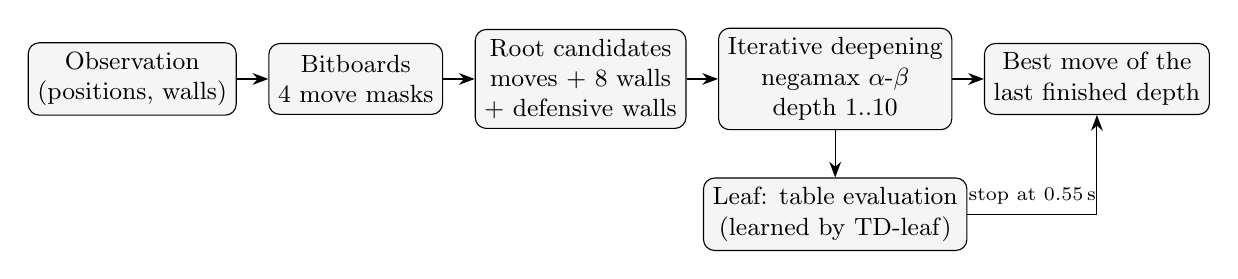
\begin{tikzpicture}[node distance=3mm and 4mm, every node/.style={font=\small},
  box/.style={draw, rounded corners, align=center, minimum height=9mm, fill=gray!8},
  arr/.style={-{Stealth[length=2mm]}}]
  \node[box] (obs) {Observation\\(positions, walls)};
  \node[box, right=of obs] (bb) {Bitboards\\4 move masks};
  \node[box, right=of bb] (cand) {Root candidates\\moves + 8 walls\\+ defensive walls};
  \node[box, right=of cand] (id) {Iterative deepening\\negamax $\alpha$-$\beta$\\depth $1..10$};
  \node[box, right=of id] (out) {Best move of the\\last finished depth};
  \node[box, below=6mm of id] (leaf) {Leaf: table evaluation\\(learned by TD-leaf)};
  \draw[arr] (obs) -- (bb); \draw[arr] (bb) -- (cand); \draw[arr] (cand) -- (id);
  \draw[arr] (id) -- (out); \draw[arr] (id) -- (leaf);
  \draw[arr] (leaf.east) -| node[pos=0.25, above, font=\scriptsize]{stop at \SI{0.55}{\second}} (out.south);
\end{tikzpicture}
\caption{Decision pipeline for one move. All state is rebuilt from the observation, so the agent
keeps working if the arena restarts it.}
\label{fig:pipeline}
\end{figure}

\subsection{Board representation with bitboards}
\label{sec:bitboard}
Squares are numbered $i = 9r + c$. A set of squares is one Python integer whose bit~$i$ is
square~$i$, as in chess engines such as Stockfish \citep{stockfish}. The walls of a position are
stored as four ``can move'' masks (up, down, left, right): bit~$i$ is set if a pawn on $i$ can
step in that direction. Adding a wall clears two bits in two masks. One step of breadth-first
search (BFS) for all squares at once is then
\begin{equation}
  R' = R \;\lor\; ((R \land U) \gg 9) \;\lor\; ((R \land D) \ll 9)
       \;\lor\; ((R \land L) \gg 1) \;\lor\; ((R \land Ri) \ll 1),
  \label{eq:flood}
\end{equation}
where $R$ is the reached set and $U, D, L, Ri$ are the masks.
Profiling had shown that distance computation took 70\% of the run time. Three further tricks
reduce the number of BFS calls:
\begin{enumerate}
  \item \textbf{Backward layers.} One backward flood from the goal row gives the distance of
        every square (\code{goal\_layers}). It is cached per (goal, wall set) because many tree
        nodes share a wall set.
  \item \textbf{Incremental update after a wall} (\code{dist\_after\_wall}). A wall only
        changes distances ``behind'' its four surrounding squares. We restart the forward flood
        at the step where the path first touches those squares and stop at the first backward
        layer that is unaffected. Re-evaluating a wall therefore costs a few iterations instead
        of a full BFS.
  \item \textbf{Skipping our own BFS.} Walls that do not touch our own shortest path cannot
        lengthen it, so no BFS is run for us.
\end{enumerate}
A unit test checks that the shortcuts match a full BFS on thousands of random positions.

\subsection{Search}
\label{sec:search}
\paragraph{Candidate moves.}
A node offers every legal pawn move. It also offers up to $K = 8$ walls that lie on the
opponent's shortest path and actually lengthen it, ranked by $\Delta d_{\text{opp}} -
\Delta d_{\text{own}}$. Restricting walls to the opponent's path keeps the branching factor near
12 instead of up to 132.
At the root only, two extra kinds of candidate are added:
\begin{itemize}
  \item \emph{Defensive walls.} For each of the three most dangerous walls the opponent could
        place (each costing us at least two steps), we try our own wall that overlaps or crosses
        that position, so the opponent can no longer place it.
  \item \emph{Arena check.} Every root candidate is checked against the arena's
        \code{legal\_moves}/\code{legal\_walls} lists, so an illegal action is impossible.
\end{itemize}

\paragraph{Negamax with iterative deepening.}
The root searches depth $1, 2, \dots, 10$ until a \SI{0.55}{\second} deadline. This leaves margin
for the slower grading CPU and for inter-process communication. The tree checks the clock every
64 nodes and aborts with an exception. If the deadline falls in the middle of an iteration, a
root move that has already been \emph{proved} better than the previous best (which is searched
first) is used rather than discarded.

\paragraph{Move ordering.}
Alpha-beta prunes most when the best move comes first. We use four standard techniques:
\begin{itemize}
  \item a transposition table keyed by (side, both pawns, both wall counts, wall masks) whose
        stored best move is searched \emph{before} the other children are generated. When it
        causes a cutoff, all the wall BFS calls of that node are skipped;
  \item two killer moves per ply \citep{akl1977killer};
  \item the history heuristic \citep{schaeffer1989history} as a tie-breaker;
  \item principal-variation search with null windows \citep{marsland1982pvs}.
\end{itemize}
Together these make the engine $1.3\times$ faster at depth 5--6, with the same move chosen in
45/45 test positions.

\paragraph{Lazy leaf evaluation.}
The ``vulnerability'' term (\cref{sec:eval}) costs about ten BFS calls. At a leaf we first
compute the cheap part. If it is already below $\alpha$, only the opponent's vulnerability could
raise the score, so that term is computed first and the other is skipped when $\alpha$ still
holds (symmetrically for $\beta$).

\paragraph{Root rules found by replay analysis.}
\begin{itemize}
  \item \emph{Progress tie-break.} A bonus of $0.001$ per step gained is added at the root
        only. Without it, positions in which ``every move gets walled later'' produced equal
        scores and the agent shuffled back and forth for 50 turns while the opponent walked home.
  \item \emph{Rush when out of walls.} With no walls left, only forward moves are considered.
        Retreating cannot make the opponent's walls less dangerous.
\end{itemize}

\Cref{alg:root} summarises the root procedure.

\begin{algorithm}[!htbp]
\caption{Root procedure of \code{choose\_action} (simplified)}
\label{alg:root}
\begin{algorithmic}[1]
\State build bitboards and distances from the observation; $T_{\text{end}} \gets \text{now} + 0.55$\,s
\State $C \gets$ moves $\cup$ top-8 walls $\cup$ defensive walls, filtered by the arena's legal lists
\If{a move in $C$ reaches the goal} \Return it \EndIf
\If{no walls left} keep only forward moves in $C$ \EndIf
\State $b \gets C_1$
\For{$d = 1, \dots, 10$}
  \State score each $c \in C$ with $-\textsc{Negamax}(c, d-1)$ $+\ 0.001\cdot\text{progress}(c)$, PVS windows
  \If{deadline hit} use the partially searched winner if it beat $b$; \textbf{break} \EndIf
  \State $b \gets$ best move; move $b$ to the front of $C$
\EndFor
\State \Return $b$ \Comment{any exception $\Rightarrow$ return the shortest-distance legal move}
\end{algorithmic}
\end{algorithm}

\subsection{Evaluation function}
\label{sec:eval}
Let $p$ be the player to move and $q$ the opponent. $d_x$ is the shortest-path distance of
player~$x$ (pawns ignored), $w_x$ their remaining walls, and $u_x$ their
\emph{vulnerability}: the largest number of extra steps that one wall on the first eight steps
of their shortest path would cost them. The score seen by $p$ is
\begin{align}
  E(p) &= \tau + \sigma\, s + V(d_p, d_q, w_p) - V(d_q, d_p, w_q)
          + \nu[w_p]\, u_q - \nu[w_q]\, u_p, \label{eq:eval}\\
  V(d, d', w) &= D[\min(d,40)] + W[w][\min(d',20)] + L[w][\operatorname{clip}(d'-d,-6,6)],
  \label{eq:side}
\end{align}
where $s = +1$ if $w_q = 0$ and $d_p \le d_q$ (an uncatchable race), $s=-1$ in the mirrored
case, and $s = 0$ otherwise.
\Cref{tab:features} lists the tables: 428 parameters in total.
\begin{itemize}
  \item The \emph{lead} table $L$ teaches the agent to keep walls in reserve when it is far
        ahead. An earlier version spent nine walls while leading by 9--15 steps and then lost.
  \item The evaluation is \emph{symmetric}: swapping the players negates $E$ apart from the
        tempo constant $\tau$. Our earlier linear evaluation was not, which produced the
        odd/even bias analysed in \cref{sec:process}.
\end{itemize}

\begin{table}[!htbp]
\centering\small
\caption{Lookup tables of the evaluation (\cref{eq:eval,eq:side}).}
\label{tab:features}
\begin{tabularx}{\linewidth}{@{}l r X@{}}
\toprule
Table & Entries & Meaning \\
\midrule
$D[d]$ & 41 & value of being $d$ steps from the goal \\
$W[w][d']$ & $11\times21$ & value of holding $w$ walls when the opponent is $d'$ steps away \\
$L[w][\ell]$ & $11\times13$ & bonus for a lead of $\ell\in[-6,6]$ steps while holding $w$ walls \\
$\nu[w]$ & 11 & weight of the opponent's vulnerability when we hold $w$ walls \\
$\tau,\ \sigma$ & 2 & tempo for the side to move; safe-race bonus \\
\midrule
Total & 428 & \\
\bottomrule
\end{tabularx}
\end{table}

\subsection{Learning the evaluation}
\label{sec:learning}
\paragraph{Stage 1: evolution of a linear evaluation.}
The first evaluations were linear in seven features. Their weights were found with a $(1+\lambda)$
evolution strategy \citep{beyer2002es}, with $\lambda = 6$ mutants per generation and
self-adaptive step size. A mutant replaced the champion only if it:
\begin{enumerate}
  \item beat the champion in side-swapped games (score at least 0.55);
  \item passed a fresh confirmation match;
  \item was not worse against a pool of older champions and fixed sparring bots.
\end{enumerate}

\paragraph{Stage 2: TD-leaf($\lambda$) on lookup tables.}
The linear formula was rewritten exactly as the tables of \cref{tab:features}, so the starting
point played identically. The tables were then refined with TD-leaf($\lambda$)
\citep{sutton1988td,baxter2000tdleaf}, as follows:
\begin{enumerate}
  \item The agent plays itself using its own negamax at depth 5--6.
  \item Each position is scored as $v = \operatorname{sigmoid}(E/K)$ at the leaf of the
        principal variation.
  \item Every table entry active at that leaf is moved by $\eta\, e_t$, with
        $e_t = \sum_k \lambda^k (v_{t+k+1} - v_{t+k})$, $\lambda = 0.7$.
\end{enumerate}
The run used 20 rounds of 200 games and about 5 minutes per round.
The learned tables can be read directly. For example, the step from distance 2 to 1 is worth
about 2.0 points versus about 1.35 far from the goal, and $\nu[w]$ rises from 0.75 with one wall
to 1.18 with six or seven.
Because the submission may not read files, the tables are written into the
\code{WEIGHTS BEGIN/END} block of the source file by the training script.

\subsection{Robustness}
\begin{itemize}
  \item The whole body of \code{choose\_action} is wrapped in \code{try/except}. Any failure
        returns the legal move with the smallest arena-provided distance, never an exception.
  \item No global state is required.
  \item Peak memory is 4--6\,MB.
  \item The longest move measured through the arena is \SI{0.563}{\second} on our laptop, with
        a \SI{0.55}{\second} budget.
\end{itemize}

% ===== sections/03-development.tex =====
\section{Development process}
\label{sec:process}

Development was organised as a sequence of numbered experiments (\#1--\#45) recorded in an
experiment log (\code{training/EXPERIMENTS.md}). Each entry records the hypothesis, the variants,
the measured numbers and the decision. Rejected ideas are logged too, so they are not retried.
\Cref{tab:versions} lists the versions that were adopted. Scores are
$(\text{wins} + \tfrac12\text{draws})/\text{games}$; ``Colab speed'' means the search budget was
halved to simulate the slower grading CPU (\cref{sec:protocol}).

\begin{table}[!htbp]
\centering\small
\caption{Adopted versions. ``Hard'' is the Hard AI of wrongway.app (\cref{sec:opponents}).
H2H = head-to-head against the previous adopted version.}
\label{tab:versions}
\begin{tabularx}{\linewidth}{@{}l X X@{}}
\toprule
Version (exp.) & Main change & Key measurement \\
\midrule
v0 (\#1) & greedy along the arena distance map, heuristic walls & loses to the sample \code{wall\_builder} \\
v1 (\#3) & alpha-beta, iterative deepening, tuple cells, depth $\le 4$ & beats greedy/random; still loses to \code{wall\_builder} (spends walls early) \\
v2 (\#5--6) & integer cells, frozenset of blocked edges, transposition table (depth 5--6); 30 generations of weight evolution & 0.85 vs v1; only 0.17--0.23 vs Hard \\
v4 (\#15--16) & vulnerability feature $u$; defensive walls at the root & 0.52 vs Hard (120 games), 0.74 vs v2 \\
v5 (\#19--22) & bitboard BFS ($2.05\times$, same moves); partial iterations; move ordering ($1.3\times$); progress tie-break & H2H 0.60 (160 games, Colab speed); vs Hard standard start $0.35\to0.47$ \\
v6 (\#23, \#26--27) & lead/reserve term (keep walls when ahead); vulnerability over 8 steps; rush rule & H2H 0.69--0.70 (reserve); exploit bot ``funnel'' 0 wins in 80 \\
v7 (\#31--34) & symmetric evaluation + tempo; depth cap $6\to10$; incremental distances ($2.6\times$) & Hard standard start 0.75, random 0.76; H2H 0.625 (160 games) \\
v8 (\#37) & evaluation rewritten as 428-entry tables, refined by TD-leaf($\lambda$) & H2H 0.49 (200 games); Hard 0.76 (200) / 0.74 (240) \\
\textbf{v9 (\#44--45)} & \textbf{held walls valued $1.2\times$ higher in the wall table} & vs wall-hoarding bots $0.23\to0.50$ (40 games); Hard standard start 0.775 (80); H2H 0.455 (160) --- \textbf{submitted} \\
\bottomrule
\end{tabularx}
\end{table}

\subsection{The turning point: depth, not evaluation}
\label{sec:depth}
Until v6, most attempts to improve the evaluation or to search unevenly failed:
\begin{itemize}
  \item a wall quiescence search (\#7);
  \item late-move reductions (\#24);
  \item search extensions for heavy walls (\#30).
\end{itemize}
Two diagnostics explained why.

\paragraph{Depth is the bottleneck (\#29).}
Ignoring the time limit, the same evaluation searched to a fixed depth of 6, 7 and 8 plies scored
0.59, 0.55 and \textbf{0.81} against Hard from the standard start (80 games each). Eight plies are
enough to see four consecutive opponent walls. Better heuristics could not replace that.

\paragraph{The evaluation had an odd/even bias (\#31).}
The root value at depth $d$ minus the value at depth $d-1$ was $+9.7, -9.3, +9.5, -9.4$ for
$d = 3..6$ (74 positions). For comparison, one step of distance is worth about 1.38 points.
The cause was two distance weights applied relative to the side to move at the leaf: for the two
players' views of the same position, $E(p) + E(q) = -0.43\,(d_p + d_q) \approx -9$ instead of~0.
The agent's style therefore flipped with the parity of the depth it happened to reach. This
explained the back-and-forth shuffling seen in replays and the failure of every uneven-depth
technique (they compare odd and even branches).
\begin{itemize}
  \item \textbf{Fix (\#32).} Dropping the two weights and adding a tempo constant reduced the bias
        to below 0.4.
  \item \textbf{Payoff (\#33).} With the bias gone, a deeper cap finally helped: Hard
        standard-start score rose from 0.56 to 0.70 with cap 8. Cap 10 was kept.
\end{itemize}
From then on, effort went into speed (\#34, $2.6\times$ with identical candidate sets).

\subsection{A standard-start weakness: undervalued walls (\#44--45)}
\label{sec:walls}
Two bots from our own team (\code{dtest2}, \code{Phat\_test2}) share 95\% of their code and hold
their walls for later. Other teams were known to follow the same idea, so we treated them as a
proxy for that style.
\begin{itemize}
  \item \textbf{The problem.} From the standard start, with both sides at simulated grading speed
        and games played one at a time, v8 lost all 20 games against them. As first player it
        replayed the same 74-move loss every time.
  \item \textbf{Diagnosis (\#44).} A deeper search of our own (depth 9) agreed with every move
        from move 37 on, so the game was lost earlier. v8 had spent 7 of its 10 walls by move 25,
        against 3 for the opponent, and the opponent's remaining walls then pushed our path from 7
        to 13 steps.
  \item \textbf{Two things ruled out.} A fixed depth of 7 or 8 still lost as first player, so an
        opening book computed by deep search would not help. The opponent also searched
        \emph{shallower} than us (7.15 vs 8.0 plies on average), so it did not win by depth.
  \item \textbf{Conclusion.} The tables learned by self-play value a wall in hand too low against
        an opponent that, unlike our own engine, keeps its walls.
  \item \textbf{Fix (\#45).} We scaled the held-wall part of the table,
        $W[w][d] \leftarrow W[0][d] + s\,(W[w][d]-W[0][d])$. Each value of $s$ was measured on
        standard-start games at ten different time budgets, to obtain different game lines.
\end{itemize}
The results for $s = 1.0 / 1.2 / 1.4$:
\begin{itemize}
  \item against the wall-hoarding pair: 0.23 / 0.50 / 0.65 (40 games each);
  \item against Hard from the standard start: 0.75 / 0.775 / 0.625;
  \item head-to-head against $s=1$: 0.455 / 0.395 (160 games).
\end{itemize}
$s=1.4$ only exploits one style, at a cost against Hard. $s=1.2$ fixes the weakness without a
measurable loss elsewhere (0.966 vs 0.969 against eight other bots), so it was adopted.

\subsection{Rejected ideas}
\Cref{tab:rejected} lists the main rejected ideas. A recurring lesson: optimising against a single
opponent, or training at a shallower depth than the agent plays at, gives weights that do not
transfer.

\begin{table}[!htbp]
\centering\small
\caption{Main rejected ideas (all measured with the protocol of \cref{sec:protocol}).}
\label{tab:rejected}
\begin{tabularx}{\linewidth}{@{}l X X@{}}
\toprule
Idea (exp.) & Result & Reason \\
\midrule
Value network, 1-ply (\#2) & 0--5\% vs heuristic bots & learned the spurious rule ``placing walls wins'' \\
Wall quiescence (\#7) & 0.51--0.62 vs v2 & costs depth \\
Repetition penalty (\#8) & 0.45 vs v2 & treats a symptom, not the cause \\
\code{pass} in the tree (\#12--13) & 0.26--0.30 vs Hard, 0.30--0.50 vs v2 & larger tree, no gain \\
Evolution against Hard only (\#14, \#17) & better vs Hard or vs alpha-beta bots, never both & over-fits one opponent; trained at depth 4 \\
Late-move reductions (\#24) & 0.35 vs previous & reduced moves were exactly the trap walls \\
Wall-pair trap search (\#25) & +0.14 vs Hard standard start, $-0.10$ random & not better everywhere \\
Heavy-wall extensions (\#30, \#33) & 0.33--0.38 vs previous & uneven depth \\
Re-evolution after v7 (\#35) & 1 of 14 generations accepted; H2H 0.47 & weights already at a local optimum \\
TD at depth 2--3 (\#36) & H2H 0.34 & depth mismatch between training and play \\
TD ``stance'' tables, +202 params (\#38) & H2H 0.44 (120 games) & no gain, 4--5\% slower \\
AlphaZero-style policy/value nets (\#39--41) & best 0.49 vs MSSV (60 games) & too little self-play data in a pure-Python budget \\
Shared wall-effect cache (\#42) & identical moves, same speed & cache hit rate only 29\% \\
Keep TT and caches across moves (\#43) & average depth 6.36 vs 6.59 & the last iteration dominates the time \\
Opening book from deep search (\#44) & depth 7--8 still loses the same opening & problem is evaluation, not depth \\
Wall scale $s=1.4$ (\#45) & 0.625 vs Hard, H2H 0.395 & exploits one style only \\
\bottomrule
\end{tabularx}
\end{table}

\subsection{AI-assisted variant pipeline}
\label{sec:pipeline}
The course allows AI tools. We used an AI coding assistant (Claude Code by Anthropic) throughout
the project. The team set the goals and made every adoption decision. The assistant wrote most
variants, ran the measurements and kept the log. Every change to the submitted file was reviewed,
and the team can explain it. The pipeline was:
\begin{enumerate}
  \item \textbf{Hypothesis from failures.} Losing games were saved as replays. The position
        before the mistake was rebuilt, and the root scores of every candidate were printed at
        each depth. Examples: the 50-turn shuffling (\#22) and the odd/even bias (\#31).
  \item \textbf{Variant generation.} The assistant implemented each hypothesis as a copy of the
        current agent behind a flag or parameter, for example \code{PROGRESS\_BONUS}
        $\in\{0.001, 0.2\}$ or \code{VULN\_STEPS} $\in\{4, 8, \infty\}$. Parameter sweeps usually
        produced 2--5 files at once. Optimisation-only changes were also checked for identical
        moves with a fixed hash seed.
  \item \textbf{Static gates.}
        \begin{itemize}
          \item Unit tests: the simulated rules must match the arena's moves, legal walls and
                distances on more than 500 random positions; self-play must stay legal; the
                agent must take an immediate win.
          \item A submission checker: both sides against the three sample bots, zero
                timeouts/errors, and the longest move time reported.
        \end{itemize}
  \item \textbf{Measurement} with the gauntlet of \cref{sec:protocol}: 40--240 games per
        opponent, at simulated grading speed.
  \item \textbf{Selection criteria.} A variant was adopted only if
        \begin{enumerate}[label=(\alph*)]
          \item it was not worse than the current champion head-to-head beyond noise (about one
                standard deviation, \cref{sec:protocol});
          \item it was not worse against Hard, from both the standard start and random openings;
          \item it still won the standard-start games against every sparring bot;
          \item it was clearly better somewhere.
        \end{enumerate}
        When two versions were equal, the simpler one was kept (\#38).
\end{enumerate}

\paragraph{Scale.}
\begin{itemize}
  \item 45 logged experiments containing about 100 hand-designed variants.
  \item Five evolution runs: 86 generations of 6 mutants, i.e.\ about 500 weight vectors, each
        judged on several dozen games.
  \item Three TD-leaf runs (14\,400, 4\,000 and 4\,000 self-play games).
  \item Three AlphaZero-style runs.
\end{itemize}
In total the agent played tens of thousands of games during development.

% ===== sections/04-evaluation.tex =====
\section{Evaluation method and results}
\label{sec:evaluation}

\subsection{Protocol}
\label{sec:protocol}
Games are played with the instructor's arena, which runs each agent in its own process and
enforces the action format. Our gauntlet tool plays games in \emph{pairs}: the same seed is
played twice with the sides swapped, so neither agent profits from moving first.
\begin{itemize}
  \item \textbf{Random openings.} Most agents are deterministic. Each pair therefore starts with
        two random plies so that different pairs give different games. The seed list is fixed
        (2026, plus 777 for confirmation), so two candidates face the same openings.
  \item \textbf{Standard start.} Seasons are played only from the standard position, so every
        candidate is also tested there. This catches fixed losing lines that random openings
        hide.
  \item \textbf{Simulated grading speed.} Our laptop (Intel i5-11400H) is about $2\times$ faster
        than a Colab CPU. ``Colab speed'' therefore runs our agent with a
        \SI{0.275}{\second} budget instead of \SI{0.55}{\second}. Opponents keep their own time,
        which makes the test pessimistic for us.
  \item \textbf{Noise.} The standard error of a score $s$ over $n$ games is
        $\sqrt{s(1-s)/n}\le 0.5/\sqrt{n}$: about $\pm0.08$ for 40 games and $\pm0.04$ for 160.
        Differences below about one standard error were treated as noise, and important
        decisions were confirmed on a second seed.
  \item \textbf{Identical-move checks.} Pure speed-ups must not change behaviour. They were
        checked with a fixed \code{PYTHONHASHSEED} and fixed depth on 40--3\,000 positions.
\end{itemize}

\subsection{Opponents}
\label{sec:opponents}
\begin{itemize}
  \item \textbf{Course sample bots:} \code{greedy}, \code{random\_agent}, \code{wall\_builder}.
  \item \textbf{Bots shared in our arena by team members and classmates:}
        \code{agent}, \code{HuynhDuy\_test2}, \code{Phat\_test1}, \code{Chubee},
        \code{duytest} (MCTS), \code{chuong-alpha-beta}, \code{dtest2} and \code{Phat\_test2}
        (the wall-hoarding pair of \cref{sec:walls}), and \code{az\_agent\_std1} (our previous
        engine plus an AlphaZero-style policy network).
  \item \textbf{A friendly-match bot from another team:} \code{mcts\_agent} (MCTS with tree reuse,
        \SI{0.70}{\second}/move).
  \item \textbf{Our own earlier versions:} \code{v2\_trained} and \code{v7\_linear}
        (\cref{tab:versions}).
  \item \textbf{An exploit bot}, \code{funnel}. It builds a wall funnel in front of our goal and
        a private corridor, modelled on a strategy shown to the class.
  \item \textbf{External programs:}
        \begin{itemize}
          \item the Hard AI of wrongway.app, run offline with the author's permission for
                private testing only;
          \item the MCTS agent of \citet{gorisanson} at its Novice, Average and Strong levels
                (2.5k/7.5k/60k rollouts, about 1/3/21\,s per move).
        \end{itemize}
\end{itemize}

\subsection{Results of the submitted version}
\Cref{tab:final} gives the final evaluation of the submitted file (v9) against 16 opponents:
160 standard-start games at real speed and 640 random-opening games at Colab speed.
\Cref{tab:external} gives the results against the external programs.

\begin{table}[!htbp]
\centering\small
\caption{Final evaluation of the submitted agent (v9). W/D/L from our point of view; score
$=(W+D/2)/n$. Standard start: 5 side-swapped pairs at \SI{0.55}{\second}/move. Random openings:
20 pairs (seed 2026) at simulated Colab speed (\SI{0.275}{\second}/move).}
\label{tab:final}
\begin{tabular}{@{}l rrr r rrr r@{}}
\toprule
& \multicolumn{4}{c}{Standard start (10 games)} & \multicolumn{4}{c}{Random openings, Colab speed (40)} \\
\cmidrule(lr){2-5}\cmidrule(l){6-9}
Opponent & W & D & L & Score & W & D & L & Score \\
\midrule
\code{greedy}            & 10 & 0 & 0 & 1.00 & 40 & 0 & 0 & 1.00 \\
\code{random\_agent}     & 10 & 0 & 0 & 1.00 & 40 & 0 & 0 & 1.00 \\
\code{wall\_builder}     & 10 & 0 & 0 & 1.00 & 40 & 0 & 0 & 1.00 \\
\code{agent}             & 10 & 0 & 0 & 1.00 & 38 & 2 & 0 & 0.97 \\
\code{HuynhDuy\_test2}   & 10 & 0 & 0 & 1.00 & 40 & 0 & 0 & 1.00 \\
\code{Phat\_test1}       & 10 & 0 & 0 & 1.00 & 40 & 0 & 0 & 1.00 \\
\code{Chubee}            & 10 & 0 & 0 & 1.00 & 38 & 2 & 0 & 0.97 \\
\code{duytest} (MCTS)    & 10 & 0 & 0 & 1.00 & 38 & 0 & 2 & 0.95 \\
\code{chuong-alpha-beta} & 10 & 0 & 0 & 1.00 & 34 & 5 & 1 & 0.91 \\
\code{mcts\_agent} (other team) &  9 & 0 & 1 & 0.90 & 36 & 2 & 2 & 0.93 \\
\code{dtest2}            &  3 & 0 & 7 & \textbf{0.30} & 32 & 0 & 8 & 0.80 \\
\code{Phat\_test2}       &  7 & 0 & 3 & 0.70 & 30 & 0 & 10 & 0.75 \\
\code{az\_agent\_std1}   &  4 & 3 & 3 & 0.55 &  9 & 9 & 22 & \textbf{0.34} \\
\code{funnel} (exploit)  & 10 & 0 & 0 & 1.00 & 40 & 0 & 0 & 1.00 \\
\code{v2\_trained} (ours)&  9 & 0 & 1 & 0.90 & 37 & 0 & 3 & 0.93 \\
\code{v7\_linear} (ours) &  5 & 0 & 5 & 0.50 & 18 & 5 & 17 & 0.51 \\
\midrule
Total & 137 & 3 & 20 & 0.87 & 550 & 25 & 65 & 0.88 \\
\bottomrule
\end{tabular}
\end{table}

\begin{table}[!htbp]
\centering\small
\caption{Results against external programs. Hard, 80 games: submitted version (v9), standard
start, Colab speed. Hard, 200/240 games: v8 (\#37). gorisanson MCTS: measured with v4 at
\SI{0.55}{\second}/move.}
\label{tab:external}
\begin{tabular}{@{}l l r r@{}}
\toprule
Opponent & Setting & Games & Score \\
\midrule
wrongway.app Hard (v9) & standard start, Colab speed & 80 & 0.775 \\
wrongway.app Hard (v8) & standard start / random, Colab speed & 200 / 240 & 0.76 / 0.74 \\
gorisanson MCTS Novice & random openings / standard start & 40 / 40 & 0.97 / 0.95 \\
gorisanson MCTS Average & random openings & 20 & 0.65 \\
gorisanson MCTS Strong & standard start & 2 & 2 wins \\
\bottomrule
\end{tabular}
\end{table}

\paragraph{Observations.}
\begin{itemize}
  \item Against 11 of the 16 opponents in \cref{tab:final} the agent scores at least 0.90 in
        both settings, including the other team's \code{mcts\_agent}. Against the course sample
        bots, the exploit bot and six of the team and classmate bots it does not lose a single
        standard-start game.
  \item The weakest results are against the wall-hoarding pair. With random openings v9 now beats
        \code{dtest2} 0.80 (v8: 0.65). From the standard start the result still depends on
        timing: 0.30 here (games run six at a time), 0.50 over the ten time budgets of \#45. This
        is the main known risk before the season.
  \item Against our own earlier engines (\code{v7\_linear}, \code{az\_agent\_std1}) v9 is even
        or slightly worse (0.34 with random openings against \code{az\_agent\_std1}). This is the
        trade-off accepted in \#45: valuing walls more helps against other styles but not against
        our own.
  \item Against the Hard AI the agent improved from 0.17--0.23 (v2) to 0.775 from the standard
        start (\cref{tab:versions,tab:external}).
  \item The submission checker reports no timeout, error or illegal action on either side. The
        longest single move measured through the arena is \SI{0.578}{\second} for a
        \SI{0.55}{\second} budget.
\end{itemize}

% ===== sections/05-conclusion.tex =====
\section{Discussion, limitations and conclusion}
\label{sec:conclusion}

\paragraph{What worked.}
The measurable gains came from three sources:
\begin{itemize}
  \item searching deeper per second: bitboards, incremental distances, move ordering;
  \item removing a systematic bias from the evaluation;
  \item a few targeted rules found by reading replays: the progress tie-break, the rush rule
        and defensive walls.
\end{itemize}
Each of these fixed a concrete, reproducible failure. Learning the evaluation with TD-leaf gave
an interpretable evaluation of equal strength rather than a stronger one. Under this search
regime, adding more static information to the evaluation did not change results (\#35, \#37,
\#38).
Pure self-play has a blind spot: the agent only learns how much a held wall is worth against
itself. Testing against bots with a different style (\#44--45) exposed this, and a one-parameter
correction fixed it.

\paragraph{Limitations and threats to validity.}
\begin{itemize}
  \item \emph{Grading speed is simulated.} The instructor confirmed that grading runs on a free
        Colab CPU and that the one-second limit includes inter-process communication. We assume
        that machine is about $2\times$ slower than our laptop (Intel i5-11400H); this ratio has
        not been measured on Colab itself. Most tests slow down only our agent, which is
        pessimistic for us; the key standard-start tests slow down both agents.
  \item \emph{Noise.} With 40 games the standard error of a score is about 0.08, and several
        decisions rest on differences of 0.05--0.10. Where possible we repeated runs on a second
        seed and pooled 160--240 games.
  \item \emph{Standard start is nearly deterministic.} Two deterministic agents produce only two
        distinct standard-start games, varied only by timing. A fixed losing line could
        therefore exist against an unseen opponent even though random-opening results are good.
  \item \emph{Horizon effect.} The agent still sometimes delays when one wall would hurt it
        badly. Defensive walls cover single-wall traps only, and only at the root.
  \item \emph{Opponent pool.} The pool contains our own earlier versions, so it may favour
        styles similar to ours. External programs (Hard, gorisanson's MCTS) reduce but do not
        remove this bias.
\end{itemize}

\paragraph{Conclusion.}
Our answer to the research question: under a one-second pure-Python budget, the strongest
design we found was a fast, well-ordered alpha-beta search with a symmetric evaluation that is
cheap enough to keep depth high, plus testing against opponents of other styles. The submitted
agent scores 0.87 from the standard start and 0.88 with random openings against 16 opponents,
and 0.775 from the standard start against wrongway.app's Hard AI at simulated grading speed. Its
main known weakness is still the standard start against wall-hoarding bots, where the result
depends on timing.
Depth~8 would win 0.81 against Hard, but two further speed-up attempts (\#42--43) gave no gain,
and a parallel search is not worthwhile on the single physical core of a free Colab CPU. The most
promising future work is therefore to learn the evaluation against a diverse pool of opponents
rather than by self-play alone.


\bibliographystyle{plainnat}
\bibliography{refs}

\appendix
% ===== sections/99-appendix.tex =====
\section{Reproducing the results}
\label{app:repro}
All commands run from the project root. The arena code is the instructor's, unmodified.
\begin{itemize}
  \item Rules and timing tests: \code{python -m unittest discover tests}
  \item Submission check (both sides, sample bots, longest move):\\
        \code{python tools/check\_submission.py TeamLeaderStudentID.py}
  \item Gauntlet (paired seeds, side swap, two random opening plies):\\
        \code{python training/gauntlet.py <bot> <opponents...>}\\
        \code{\ \ \ \ --pairs 20 --workers 6 --seed 2026}\\
        add \code{--opening 0} for the standard start.
  \item Simulated grading speed: a copy of the agent with \code{TIME\_BUDGET = 0.275}.
  \item Training: \code{training/evolve.py} (evolution of the linear evaluation),
        \code{training/td\_learn.py} (TD-leaf($\lambda$) on the tables; writes the
        \code{WEIGHTS} block).
\end{itemize}

\section{Statement on the use of AI tools and third-party code}
\begin{itemize}
  \item An AI coding assistant (Claude Code, Anthropic) was used to implement variants, run
        experiments and draft documentation, as described in \cref{sec:pipeline}. The team
        reviewed all submitted code and can explain every part of it.
  \item No code from other students or from third-party programs is included in the
        submission.
  \item The wrongway.app Hard AI was run only offline, for private testing, with the permission
        of its author; its code is not distributed with this work.
  \item The MCTS program of \citet{gorisanson} (MIT licence) was used only as a test opponent.
\end{itemize}


\end{document}
